\documentclass[11pt,a4paper]{article}

% ------------------------------------------------------------------
% Packages
% ------------------------------------------------------------------
\usepackage[T1]{fontenc}
\usepackage[utf8]{inputenc}
\usepackage{lmodern}
\usepackage[margin=2.4cm]{geometry}
\usepackage{amsmath,amssymb}
\usepackage{graphicx}
\usepackage{booktabs}
\usepackage{longtable}
\usepackage{array}
\usepackage{enumitem}
\usepackage{xcolor}
\usepackage{listings}
\usepackage{titlesec}
\usepackage{fancyhdr}
\usepackage{caption}
\usepackage{hyperref}
\usepackage{tikz}
\usetikzlibrary{arrows.meta,positioning,shapes.geometric,fit,backgrounds}

% ------------------------------------------------------------------
% Hyperref
% ------------------------------------------------------------------
\hypersetup{
  colorlinks=true,
  linkcolor=blue!50!black,
  urlcolor=blue!50!black,
  citecolor=blue!50!black,
  pdftitle={PetroLumen -- Reservoir Module: Free/Open Implementation Guide},
  pdfauthor={PetroLumen Project}
}

% ------------------------------------------------------------------
% Headers
% ------------------------------------------------------------------
\pagestyle{fancy}
\fancyhf{}
\fancyhead[L]{\small PetroLumen}
\fancyhead[R]{\small Reservoir Module --- Implementation Guide}
\fancyfoot[C]{\thepage}
\renewcommand{\headrulewidth}{0.4pt}

% ------------------------------------------------------------------
% Listings
% ------------------------------------------------------------------
\definecolor{codebg}{RGB}{247,247,250}
\definecolor{codekw}{RGB}{0,90,160}
\definecolor{codestr}{RGB}{140,60,20}
\definecolor{codecom}{RGB}{90,120,90}

\lstdefinestyle{py}{
  language=Python,
  backgroundcolor=\color{codebg},
  basicstyle=\ttfamily\small,
  keywordstyle=\color{codekw}\bfseries,
  stringstyle=\color{codestr},
  commentstyle=\color{codecom}\itshape,
  numbers=left,
  numberstyle=\tiny\color{gray},
  numbersep=8pt,
  frame=single,
  rulecolor=\color{gray!40},
  breaklines=true,
  breakatwhitespace=false,
  showstringspaces=false,
  tabsize=4,
  captionpos=b
}

\lstdefinestyle{sh}{
  language=bash,
  backgroundcolor=\color{codebg},
  basicstyle=\ttfamily\small,
  keywordstyle=\color{codekw}\bfseries,
  commentstyle=\color{codecom}\itshape,
  frame=single,
  rulecolor=\color{gray!40},
  breaklines=true,
  showstringspaces=false,
  captionpos=b
}

\lstdefinestyle{txt}{
  backgroundcolor=\color{codebg},
  basicstyle=\ttfamily\small,
  frame=single,
  rulecolor=\color{gray!40},
  breaklines=true,
  showstringspaces=false,
  captionpos=b
}

\lstset{style=py}

% ------------------------------------------------------------------
% Section styling
% ------------------------------------------------------------------
\titleformat{\section}{\Large\bfseries\color{blue!40!black}}{\thesection}{0.8em}{}
\titleformat{\subsection}{\large\bfseries\color{blue!30!black}}{\thesubsection}{0.6em}{}

% ------------------------------------------------------------------
% Title
% ------------------------------------------------------------------
\title{
  \vspace{-1.5cm}
  \textbf{PetroLumen}\\[0.3em]
  \large Reservoir Module --- Free and Open Implementation Guide\\[0.5em]
  \normalsize A zero-licence-cost build plan for a modular,\\
  Python-first reservoir engineering workbench
}
\author{PetroLumen Engineering}
\date{\today}

\begin{document}
\maketitle
\thispagestyle{empty}

\begin{abstract}
\noindent
This document specifies how to design, build, integrate, validate and ship the
\textbf{reservoir module} of \emph{PetroLumen} using only free and open-source
software. It covers the module's scope, its place in the wider suite, the
concrete tool stack (OPM Flow, resqpy, Petres, GeostatsPy, pyResToolbox,
PetroCalc, welltest-pta, JutulDarcy, PyVista, ResInsight, and friends), the data
model, integration patterns, a phased roadmap, a validation programme against
public benchmarks, and the licensing obligations that come with an
open-source dependency graph. The goal is not to clone a commercial simulator
line-by-line, but to reach a defensible, transparent engineering level for
conventional reservoir work at zero software cost.
\end{abstract}

\tableofcontents
\clearpage

% ==================================================================
\section{Scope and design principles}
% ==================================================================

\subsection{What the reservoir module owns}
The reservoir module is the \emph{subsurface physics and forecasting core} of
PetroLumen. It owns:
\begin{itemize}[leftmargin=1.4em]
  \item reservoir fluid characterisation (PVT) and rock--fluid data;
  \item volumetrics, material balance and drive-mechanism analysis;
  \item pressure transient analysis (well testing);
  \item static model ingestion, upscaling and grid handling;
  \item numerical simulation (black-oil, compositional where feasible);
  \item results post-processing, forecasting and uncertainty;
  \item the canonical reservoir data model exposed to other modules
        (production, economics, reporting).
\end{itemize}

It explicitly does \emph{not} own drilling, completions design, surface
facilities, fiscal modelling or corporate reporting; those are sibling
modules that consume the reservoir module's outputs through a stable API.

\subsection{Design principles}
\begin{enumerate}[leftmargin=1.4em]
  \item \textbf{Free at runtime.} No component of the module may require a
        paid licence to execute. Commercial tools may be supported as
        optional importers/exporters only.
  \item \textbf{Transparent internals.} Every equation used for a result must
        be traceable to a function, a paper or a textbook reference.
  \item \textbf{Open standards first.} RESQML for model exchange, Eclipse-style
        decks for simulation I/O, LAS for well logs, CSV/Parquet for tabular
        data.
  \item \textbf{Modular boundaries.} Each engineering discipline is a separate
        package with a typed interface; the UI never imports solver internals.
  \item \textbf{Reproducibility.} Every run stores its inputs, deck, solver
        version and environment hash.
  \item \textbf{Validate before you trust.} No module ships without passing a
        public benchmark suite.
\end{enumerate}

% ==================================================================
\section{Architecture of the module}
% ==================================================================

\subsection{Layer diagram}

\begin{figure}[htbp]
\centering
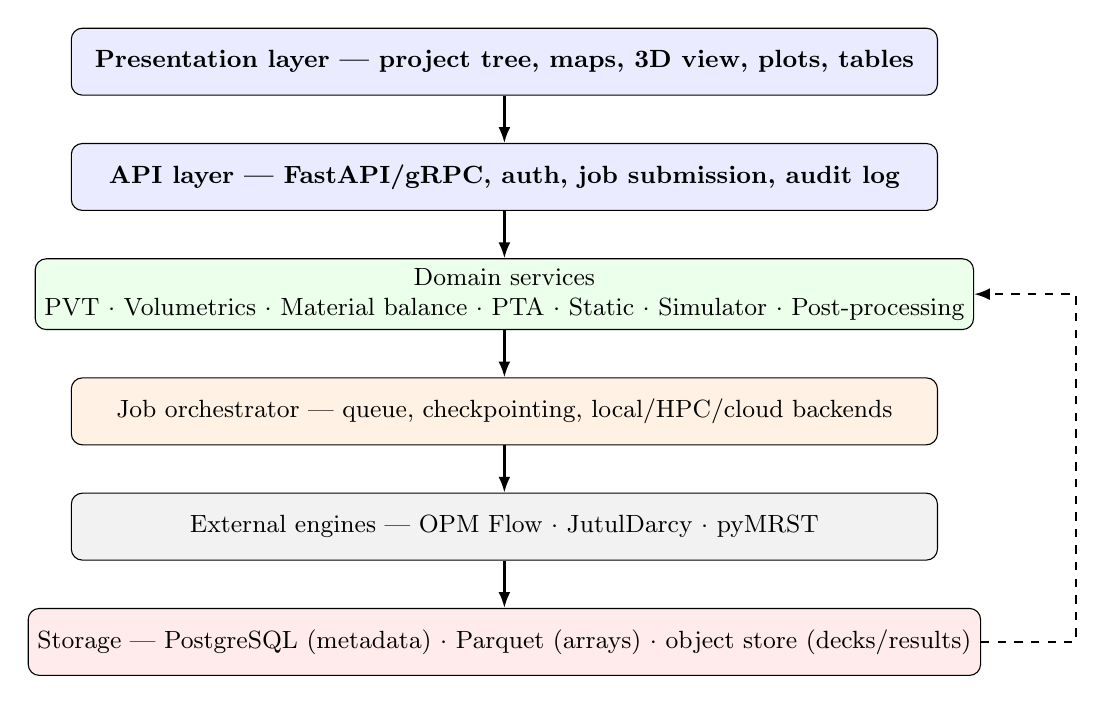
\begin{tikzpicture}[
  node distance=6mm,
  box/.style={draw, rounded corners, align=center, minimum width=11cm,
              minimum height=0.85cm, font=\small},
  layer/.style={draw, rounded corners, align=center, minimum width=11cm,
                minimum height=0.85cm, font=\small\bfseries},
  arr/.style={-{Latex[length=2mm]}, thick}
]
\node[layer, fill=blue!8] (ui) {Presentation layer --- project tree, maps, 3D view, plots, tables};
\node[layer, fill=blue!8, below=of ui] (api) {API layer --- FastAPI/gRPC, auth, job submission, audit log};
\node[box, fill=green!8, below=of api] (dom) {Domain services\\PVT $\cdot$ Volumetrics $\cdot$ Material balance $\cdot$ PTA $\cdot$ Static $\cdot$ Simulator $\cdot$ Post-processing};
\node[box, fill=orange!10, below=of dom] (orch) {Job orchestrator --- queue, checkpointing, local/HPC/cloud backends};
\node[box, fill=gray!10, below=of orch] (ext) {External engines --- OPM Flow $\cdot$ JutulDarcy $\cdot$ pyMRST};
\node[box, fill=red!8, below=of ext] (store) {Storage --- PostgreSQL (metadata) $\cdot$ Parquet (arrays) $\cdot$ object store (decks/results)};

\draw[arr] (ui) -- (api);
\draw[arr] (api) -- (dom);
\draw[arr] (dom) -- (orch);
\draw[arr] (orch) -- (ext);
\draw[arr] (ext) -- (store);
\draw[arr, dashed] (store.east) -- ++(1.2,0) |- (dom.east);
\end{tikzpicture}
\caption{Layered architecture of the PetroLumen reservoir module. Solid arrows
are request flow; the dashed arrow is the results feedback path.}
\label{fig:arch}
\end{figure}

\subsection{Domain packages}
Each bullet below becomes a Python package under \texttt{petrolumen/reservoir/}.

\begin{longtable}{@{}p{3.3cm}p{4.2cm}p{7.4cm}@{}}
\toprule
\textbf{Package} & \textbf{Responsibility} & \textbf{Primary free dependency}\\
\midrule
\endhead
\texttt{fluids}      & PVT tables, correlations, lab matching & pyResToolbox, PetroCalc\\
\texttt{volumetrics} & OOIP/OGIP, drive indices, recovery factors & PetroCalc, NumPy\\
\texttt{matbal}      & Material balance, aquifer models & SciPy, custom\\
\texttt{pta}         & Pressure transient analysis & welltest-pta, pta-learn\\
\texttt{static}      & Grids, upscaling, property models & Petres, GeostatsPy, resqpy\\
\texttt{sim}         & Deck generation, run control, parsing & OPM Flow, resqpy, ecl-reader\\
\texttt{post}        & Forecasting, aggregation, visualisation & pandas, xarray, PyVista\\
\texttt{uncertainty} & Ensembles, sensitivity, assisted HM & SciPy, scikit-learn, SALib\\
\texttt{core}        & Data model, units, validation & pydantic, pint\\
\bottomrule
\end{longtable}

% ==================================================================
\section{The free tool stack}
% ==================================================================

\subsection{Mapping concerns to tools}

\begin{longtable}{@{}p{3.6cm}p{3.4cm}p{2.2cm}p{5.6cm}@{}}
\toprule
\textbf{Concern} & \textbf{Tool} & \textbf{Licence} & \textbf{Role in PetroLumen}\\
\midrule
\endhead
Simulation engine   & OPM Flow          & OSL-3.0 / GPL parts & Full-field black-oil and compositional runs from Eclipse-style decks\\
Simulation (Julia)  & JutulDarcy.jl     & MIT                & Alternative engine, fast prototyping, differentiable workflows\\
Simulation (Python) & pyMRST / MRST     & GPL-3.0            & Research-grade methods, teaching, custom discretisations\\
Grid handling       & Petres            & LGPL               & Corner-point grids, \texttt{.GRDECL} read/write, in-app 3D\\
Open model exchange & resqpy            & Apache-2.0         & RESQML read/write, HDF5-backed model store\\
Geostatistics       & GeostatsPy        & MIT                & Kriging, SGS, spatial interpolation\\
PVT / correlations  & pyResToolbox      & GPL-3.0            & Fluid property routines\\
Broad calculations  & PetroCalc         & MIT                & Material balance, IPR, economics, unit helpers\\
Well testing        & welltest-pta      & MIT                & Bourdet derivative, Horner, parameter estimation\\
Well testing (auto) & pta-learn         & MIT                & Transient and flow-regime detection\\
Nodal analysis      & pynodal / rNodal  & MIT                & IPR/VLP for hand-off to production module\\
Numerical arrays    & NumPy, SciPy      & BSD                & Linear algebra, ODE/PDE helpers\\
Tabular / labelled  & pandas, xarray    & BSD / Apache       & Time series, gridded results\\
Visualisation       & PyVista, matplotlib & MIT / PSF        & 3D grids, 2D plots\\
3D review (external) & ResInsight       & GPL-3.0            & Optional large-model viewer\\
Uncertainty         & SALib, scikit-learn & MIT / BSD        & Sensitivity, sampling, surrogates\\
Units               & pint              & BSD                & Unit-safe engineering quantities\\
Schema / validation & pydantic          & MIT                & Typed domain objects\\
API                 & FastAPI           & MIT                & HTTP service layer\\
Jobs                & Celery or RQ      & BSD                & Local and cluster job queue\\
Database            & PostgreSQL        & PostgreSQL licence & Metadata, audit, provenance\\
\bottomrule
\end{longtable}

\subsection{Licensing implications}
Three dependencies shape PetroLumen's licence strategy:
\begin{itemize}[leftmargin=1.4em]
  \item \textbf{GPL components (pyResToolbox, MRST, ResInsight)} must be used
        as \emph{separate processes} invoked over a subprocess or service
        boundary if PetroLumen itself is to remain permissively licensed.
        Bundling them into the same address space triggers copyleft.
  \item \textbf{OPM Flow} is best treated as an external executable: PetroLumen
        writes decks, launches the binary, and parses results. This keeps the
        boundary clean and the engine swappable.
  \item \textbf{Apache/MIT/BSD components} (resqpy, Petres, GeostatsPy,
        welltest-pta, PyVista) can be imported directly and are safe to link.
\end{itemize}

\noindent\textbf{Recommendation.} Ship PetroLumen itself under Apache-2.0 or MIT
and declare GPL engines as \emph{optional, user-installed backends} discovered
at runtime.

% ==================================================================
\section{The reservoir data model}
% ==================================================================

\subsection{Core entities}
The module's canonical objects, defined with \texttt{pydantic} and stored in
PostgreSQL, are:

\begin{longtable}{@{}p{3.0cm}p{11.8cm}@{}}
\toprule
\textbf{Entity} & \textbf{Key fields}\\
\midrule
\endhead
\texttt{Project}   & id, name, crs, units, created, owner, tags\\
\texttt{FluidModel} & id, project\_id, type (black-oil/compositional), component table, correlations, source lab report\\
\texttt{RockModel}  & id, project\_id, relperm tables, capillary pressure, compaction\\
\texttt{Grid}       & id, project\_id, format (corner-point/CPG), path, dimensions, active mask, parent\_grid\\
\texttt{Well}       & id, project\_id, name, trajectory, perforations, schedule refs\\
\texttt{Schedule}   & id, project\_id, events (rates, pressures, controls), dates\\
\texttt{Case}       & id, project\_id, grid\_ref, fluid\_ref, rock\_ref, schedule\_ref, engine, solver options, status\\
\texttt{Run}        & id, case\_id, deck\_hash, environment\_hash, started, finished, exit\_code, output\_paths\\
\texttt{ResultSet}  & id, run\_id, kind (grid/time-series/summary), variables, time range, storage path\\
\texttt{Test}       & id, well\_id, pressure series, rate history, interpretation model, fitted params\\
\texttt{Uncertainty}& id, project\_id, priors, sampler, ensemble\_size, runs\\
\bottomrule
\end{longtable}

\subsection{Typed domain object example}

\begin{lstlisting}[caption={A pydantic model for a simulation case (excerpt).}]
from datetime import datetime
from enum import Enum
from typing import Optional
from pydantic import BaseModel, Field

class Engine(str, Enum):
    OPM_FLOW = "opm_flow"
    JUTULDARCY = "jutuldarcy"
    PYMRST = "pymrst"

class Case(BaseModel):
    id: str
    project_id: str
    name: str
    grid_id: str
    fluid_id: str
    rock_id: str
    schedule_id: str
    engine: Engine = Engine.OPM_FLOW
    solver: dict = Field(default_factory=dict)
    created: datetime
    parent_case: Optional[str] = None

    class Config:
        use_enum_values = True
\end{lstlisting}

\subsection{Storage split}
\begin{itemize}[leftmargin=1.4em]
  \item \textbf{PostgreSQL} --- entities above, audit log, provenance, user
        metadata.
  \item \textbf{Parquet} --- time series (well rates, pressures, summary
        vectors) partitioned by run and variable.
  \item \textbf{Object store / filesystem} --- Eclipse decks, RESQML/HDF5
        models, restart files, full 3D result arrays.
\end{itemize}

% ==================================================================
\section{Module-by-module implementation}
% ==================================================================

Each subsection states: purpose, free tooling, the interface PetroLumen exposes,
and the key pitfalls.

\subsection{Fluids and PVT}
\textbf{Purpose.} Provide consistent fluid properties to volumetrics,
material balance and the simulator.

\textbf{Tooling.} \texttt{pyResToolbox} for correlations (Standing, Vasquez--Beggs,
Hall--Yarborough, etc.) and \texttt{PetroCalc} for higher-level helpers. Store
the resulting tables as immutable, versioned \texttt{FluidModel} objects so
every downstream calculation can cite the exact table used.

\textbf{Interface.}
\begin{lstlisting}[caption={Fluids package contract.}]
class FluidProvider(Protocol):
    def rs(self, p: float, t: float) -> float: ...
    def bo(self, p: float, t: float) -> float: ...
    def mu_o(self, p: float, t: float) -> float: ...
    def to_black_oil_table(self, p_grid, t) -> "BlackOilTable": ...
\end{lstlisting}

\textbf{Pitfalls.} Correlation domains are narrow; reject inputs outside the
fitted range and require the engineer to pick an alternative or supply lab data.

\subsection{Volumetrics and material balance}
\textbf{Purpose.} Fast, pre-simulation estimates: OOIP/OGIP, drive indices,
recovery factor screening, aquifer influx.

\textbf{Tooling.} \texttt{PetroCalc} for standard formulas; \texttt{SciPy} for
non-linear aquifer fitting; custom code for Havlena--Odeh straight-line
analysis.

\textbf{Pitfalls.} Unit handling. Use \texttt{pint} everywhere and forbid raw
floats crossing module boundaries.

\subsection{Pressure transient analysis}
\textbf{Purpose.} Permeability, skin, wellbore storage, boundary and
heterogeneity inference from pressure--time data.

\textbf{Tooling.} \texttt{welltest-pta} for the full pipeline (parsing, event
detection, Bourdet derivative, Horner, radial-flow parameter estimation);
\texttt{pta-learn} for automatic transient and flow-regime detection.

\textbf{Interface.} Expose \texttt{interpret(series) -> TestInterpretation} with
the fitted model, parameters, confidence intervals and a log--log diagnostic
image.

\textbf{Pitfalls.} Garbage-in pressure data. Gate the module behind a QC step
(downsampling, outlier removal, rate alignment).

\subsection{Static model and upscaling}
\textbf{Purpose.} Ingest corner-point grids, upscale properties, build
stochastic property models.

\textbf{Tooling.} \texttt{Petres} for grid construction, \texttt{.GRDECL}
round-tripping and in-app 3D; \texttt{GeostatsPy} for kriging and sequential
Gaussian simulation; \texttt{resqpy} for RESQML.

\textbf{Pitfalls.} Coordinate-system and unit mismatches between RESQML, Eclipse
and internal grids. Normalise at ingestion, never at run time.

\subsection{Numerical simulation}
\textbf{Purpose.} The forecasting engine.

\textbf{Tooling and strategy.}
\begin{enumerate}[leftmargin=1.4em]
  \item \textbf{Primary engine: OPM Flow.} PetroLumen generates an Eclipse-style
        deck from the \texttt{Case} object, launches the binary as a subprocess,
        monitors the log, and parses \texttt{.SMSPEC}/\texttt{.UNSMRY} and
        \texttt{.EGRID}/\texttt{.INIT}/\texttt{.UNRST} outputs.
  \item \textbf{Alternative engine: JutulDarcy.jl.} Use for fast prototyping and
        differentiable workflows; call via a Julia subprocess or \texttt{juliacall}.
  \item \textbf{Research engine: pyMRST.} Enable only when the user has installed
        MRST; useful for custom discretisations and teaching.
\end{enumerate}

\textbf{Deck generation example.}
\begin{lstlisting}[caption={Minimal deck writer from a Case object.}]
def write_deck(case: Case, grid_path, out_path):
    with open(out_path, "w") as f:
        f.write("RUNSPEC\n")
        f.write("DIMENS\n 10 10 3 /\n")
        f.write("OIL\nWATER\nGAS\n")
        f.write("FIELD\n")
        f.write("GRID\n")
        f.write(f"INCLUDE\n '{grid_path}' /\n")
        f.write("PROPS\n")
        f.write(f"INCLUDE\n '{case.fluid_id}.inc' /\n")
        f.write(f"INCLUDE\n '{case.rock_id}.inc' /\n")
        f.write("SCHEDULE\n")
        f.write(f"INCLUDE\n '{case.schedule_id}.inc' /\n")
        f.write("END\n")
\end{lstlisting}

\textbf{Run wrapper.}
\begin{lstlisting}[caption={Subprocess isolation keeps the GPL boundary clean.}]
import subprocess, hashlib, json, datetime

def run_flow(deck_path, workdir, timeout=86400):
    env = {"OMP_NUM_THREADS": "8"}
    proc = subprocess.run(
        ["flow", deck_path],
        cwd=workdir, env=env, capture_output=True, text=True,
        timeout=timeout
    )
    return {
        "deck_hash": hashlib.sha256(open(deck_path, "rb").read()).hexdigest(),
        "exit_code": proc.returncode,
        "stdout_tail": proc.stdout[-4000:],
        "finished": datetime.datetime.utcnow().isoformat(),
    }
\end{lstlisting}

\textbf{Pitfalls.} Silent convergence failures; missing restart files; unit
drift between deck keywords and internal SI storage. Parse the summary file
independently of the log and cross-check total produced volumes against the
deck's initial-in-place declaration.

\subsection{Post-processing and visualisation}
\textbf{Purpose.} Turn raw runs into engineering answers.

\textbf{Tooling.} \texttt{pandas}/\texttt{xarray} for summary vectors;
\texttt{PyVista} for in-app 3D; \texttt{ResInsight} as an optional external
viewer for very large models; \texttt{matplotlib} for standard engineering
plots (rate--time, pressure--time, log--log, tornado).

\textbf{Pitfalls.} Re-inventing plotting. Standardise on a small internal plot
library so every module produces visually consistent output.

\subsection{Uncertainty and assisted history matching}
\textbf{Purpose.} Quantify forecast ranges and automate parameter calibration.

\textbf{Tooling.} \texttt{SALib} for sampling and sensitivity; \texttt{scikit-learn}
for surrogate models (random forests, Gaussian processes) trained on ensemble
runs; \texttt{SciPy} optimisers for deterministic HM; optional ensemble Kalman
or ensemble smoother implemented in-house.

\textbf{Pitfalls.} Ensembles are expensive. Cap default ensemble size, run on a
job queue, and always expose the surrogate's error metric alongside the
forecast.

% ==================================================================
\section{Integration patterns}
% ==================================================================

\subsection{Job orchestration}
Every simulation is a job with: an immutable deck, an environment manifest, a
queue entry, a status machine (\texttt{queued -> running -> finished|failed}),
and persisted outputs. Celery or RQ for local execution; the same interface
targets Slurm or Kubernetes for HPC.

\subsection{Results caching}
Key results by \texttt{(deck\_hash, engine\_version, environment\_hash)}. Identical
re-runs return cached outputs instantly; this makes parameter sweeps and
assisted HM tractable.

\subsection{Plugin contract}
Third parties extend the module through entry points:
\begin{lstlisting}[caption={Plugin interface exposed to internal and external authors.}]
# pyproject.toml
[project.entry-points."petrolumen.reservoir.engines"]
my_engine = "my_pkg.engine:MyEngine"

# contract
class EnginePlugin(Protocol):
    name: str
    def validate_case(self, case) -> list[str]: ...
    def build_inputs(self, case, workdir) -> dict: ...
    def run(self, workdir, options) -> "RunResult": ...
    def parse_results(self, workdir) -> "ResultSet": ...
\end{lstlisting}

This single contract is what makes OPM Flow, JutulDarcy and pyMRST
interchangeable behind the UI.

% ==================================================================
\section{Validation programme}
% ==================================================================

No reservoir module is credible without published benchmarks. Adopt the
following as non-negotiable regression tests.

\begin{longtable}{@{}p{2.4cm}p{5.0cm}p{6.8cm}@{}}
\toprule
\textbf{Benchmark} & \textbf{What it exercises} & \textbf{Pass criterion}\\
\midrule
\endhead
SPE1  & Three-phase, two-well, gas coning & Bottom-hole pressure and gas rate within 2\% of published reference\\
SPE9  & Black-oil, 26 wells, faulted grid & Cumulative production within 2\% at final time\\
SPE10 & Highly heterogeneous 60$\times$220$\times$85 permeability field & Water-cut history and CPU time documented; determinism across runs\\
Norne & Real field, complex geology, many wells & Summary vectors within agreed tolerance vs.\ reference run\\
\bottomrule
\end{longtable}

\noindent Additional requirements:
\begin{itemize}[leftmargin=1.4em]
  \item \textbf{Determinism.} Same deck and engine version must produce
        bit-identical summary output on the same hardware.
  \item \textbf{Unit round-trip.} Every quantity survives
        SI $\rightarrow$ field $\rightarrow$ SI without drift.
  \item \textbf{Importer round-trip.} RESQML in $\rightarrow$ internal $\rightarrow$
        RESQML out must be lossless for supported attributes (verify with \texttt{resqpy}).
  \item \textbf{Deck round-trip.} Parse an Eclipse deck, regenerate it, and
        confirm OPM Flow produces the same summary vectors.
\end{itemize}

% ==================================================================
\section{Performance strategy}
% ==================================================================

A pure-Python layer will not compete with commercial solvers on large models;
the design therefore assumes the heavy lifting is delegated.

\begin{enumerate}[leftmargin=1.4em]
  \item \textbf{Delegate numerics.} OPM Flow, JutulDarcy and PETSc-backed
        kernels carry the linear algebra; Python orchestrates.
  \item \textbf{Vectorise the glue.} Use NumPy and \texttt{xarray} for result
        aggregation; never loop over grid cells in Python.
  \item \textbf{Compile hotspots.} Numba or Cython for custom upscaling,
        derivative computation and aquifer fitting.
  \item \textbf{Parallelism by job, not thread.} Run cases concurrently on the
        queue; inside a case, let the engine manage MPI/OpenMP.
  \item \textbf{Optional GPU path.} JutulDarcy on CUDA-capable hardware where
        available; keep it optional so the default install stays portable.
\end{enumerate}

% ==================================================================
\section{Repository and delivery}
% ==================================================================

\subsection{Layout}
\begin{lstlisting}[style=txt, caption={Suggested repository layout.}]
petrolumen/
  pyproject.toml
  src/petrolumen/
    core/            # units, schema, errors, audit
    reservoir/
      fluids/
      volumetrics/
      matbal/
      pta/
      static/
      sim/
        engines/     # opm_flow.py, jutuldarcy.py, pymrst.py
        deck.py
        parse.py
      post/
      uncertainty/
    api/             # FastAPI routers
    jobs/            # queue, workers, backends
  tests/
    unit/
    integration/
    benchmarks/      # SPE1, SPE9, SPE10, Norne fixtures
  docs/
  plugins/
\end{lstlisting}

\subsection{Quality gates}
\begin{itemize}[leftmargin=1.4em]
  \item \texttt{pytest} unit and integration suites on every commit.
  \item Benchmark suite on every release candidate; failures block release.
  \item \texttt{mypy} strict typing on \texttt{core} and all public interfaces.
  \item \texttt{ruff} and \texttt{black} for style.
  \item Containerised CI that installs OPM Flow to run the integration suite.
\end{itemize}

\subsection{Distribution}
Ship as a Python package plus an optional container image that bundles the
engines. Users who prefer a permissive-only install can exclude GPL engines
via extras (\texttt{pip install petrolumen[reservoir]} vs.\
\texttt{petrolumen[reservoir,gpl-engines]}).

% ==================================================================
\section{Phased roadmap}
% ==================================================================

\begin{longtable}{@{}p{1.6cm}p{4.4cm}p{8.6cm}@{}}
\toprule
\textbf{Phase} & \textbf{Deliverable} & \textbf{Contents}\\
\midrule
\endhead
M0 & Skeleton       & Core schema, units, project store, CI, empty API\\
M1 & Engineering basics & Fluids, volumetrics, material balance, PTA; import LAS/CSV; plots\\
M2 & Simulation MVP & OPM Flow engine plugin, deck writer, parser, job queue, SPE1 and SPE9 passing\\
M3 & Static link    & RESQML via resqpy, Petres grids, upscaling, SPE10 passing\\
M4 & Post-processing & Summary and 3D parsing, PyVista viewer, forecasting, export\\
M5 & Uncertainty    & Ensembles, sensitivity, surrogate-assisted HM, Norne passing\\
M6 & Hardening      & Performance tuning, plugin SDK, documentation, container image\\
\bottomrule
\end{longtable}

\noindent A realistic solo-developer cadence is roughly one to two phases per
quarter for M0--M3, with M4--M6 depending on available engineering time.

% ==================================================================
\section{Risks and mitigations}
% ==================================================================

\begin{longtable}{@{}p{4.4cm}p{9.6cm}@{}}
\toprule
\textbf{Risk} & \textbf{Mitigation}\\
\midrule
\endhead
Validation gap versus commercial tools & Publish benchmark results transparently; state supported physics explicitly in the UI\\
GPL contamination of the product & Enforce process isolation for GPL engines; ship them as optional extras\\
Engine version drift breaking parsing & Pin engine versions per release; keep parsers behind an adapter layer\\
Performance on large models & Delegate to OPM/JutulDarcy; document supported model sizes\\
Maintainer burnout on a broad scope & Phase aggressively; ship M0--M2 before touching uncertainty\\
Data format churn (RESQML, decks) & Round-trip tests in CI; treat importers as first-class modules\\
\bottomrule
\end{longtable}

% ==================================================================
\section{Getting started today}
% ==================================================================

\begin{lstlisting}[style=sh, caption={Bootstrap environment for the reservoir module.}]
python -m venv .venv && source .venv/bin/activate
pip install pydantic pint numpy scipy pandas xarray \
            fastapi uvicorn celery redis \
            resqpy petres geostatsypy pvista \
            welltest-pta pta-learn salib scikit-learn

# Optional, GPL / external engines (install separately)
# OPM Flow:   use the official binary release or a container image
# pyResToolbox, PetroCalc: pip install and vendor as subprocess services
# JutulDarcy.jl: install Julia, then `using Pkg; Pkg.add("JutulDarcy")`
\end{lstlisting}

\noindent The first concrete milestone is M1: a user can create a project,
import a fluid and a pressure test, compute OOIP and run a material balance ---
all inside PetroLumen, all free.

% ==================================================================
\section*{References}
\addcontentsline{toc}{section}{References}
% ==================================================================

\begin{enumerate}[leftmargin=1.6em, label={[\arabic*]}]
  \item L.P. Dake, \emph{Fundamentals of Reservoir Engineering}, Elsevier, 1978.
  \item L.P. Dake, \emph{The Practice of Reservoir Engineering}, Elsevier, rev.\ ed.\ 2001.
  \item T. Ahmed, \emph{Reservoir Engineering Handbook}, Gulf Professional Publishing, 5th ed.\ 2019.
  \item W.D. McCain Jr., \emph{The Properties of Petroleum Fluids}, PennWell, 2nd ed.\ 1990.
  \item K.-A. Lie, \emph{An Introduction to Reservoir Simulation Using MATLAB/GNU Octave}, Cambridge University Press, 2019.
  \item D.W. Peaceman, \emph{Fundamentals of Numerical Reservoir Simulation}, Elsevier, 1977.
  \item T. Ertekin, J.H. Abou-Kassem, G.R. King, \emph{Basic Applied Reservoir Simulation}, SPE, 2001.
  \item M.J. Pyrcz, C.V. Deutsch, \emph{Geostatistical Reservoir Modeling}, Oxford University Press, 2nd ed.\ 2014.
  \item R.N. Horne, \emph{Modern Well Test Analysis: A Computer-Aided Approach}, Petroway, 1995.
  \item T.A.O. Ganat, \emph{Modern Pressure Transient Analysis of Petroleum Reservoirs}, Springer, 2023.
  \item B. Guo, W.C. Lyons, A. Guo, \emph{Petroleum Production Engineering: A Computer-Assisted Approach}, Gulf Professional Publishing, 2007.
  \item R. Wheaton, \emph{Fundamentals of Applied Reservoir Engineering}, Gulf Professional Publishing, 2016.
  \item A. Satter, G.M. Iqbal, J.L. Buchwalter, \emph{Practical Enhanced Reservoir Engineering}, PennWell, 2008.
  \item Y.N. Pandey et al., \emph{Machine Learning in the Oil and Gas Industry}, Apress, 2020.
  \item M.J. Pyrcz, \emph{Applied Machine Learning in Python} and \emph{Applied Geostatistics in Python}, free e-books, 2024.
  \item Open Porous Media Initiative, \emph{OPM Flow} documentation and source.
  \item Equinor, \emph{ResInsight} and \emph{JutulDarcy.jl} documentation.
  \item bp, \emph{resqpy} documentation (RESQML in Python).
  \item Society of Petroleum Engineers, comparative solution projects SPE1, SPE9, SPE10 and the Norne benchmark dataset.
\end{enumerate}

\end{document}